%!TEX program = xelatex

\documentclass[11pt,compress,aspectratio=1610]{beamer}

%\setbeameroption{show notes}

\iffalse
\setbeamertemplate{note page}{
	\rmfamily
	\underline{\insertsection -- \insertsubsection} \\
	\scriptsize
	\setbeamertemplate{itemize/enumerate body begin}{\scriptsize}
	\setbeamertemplate{itemize/enumerate subbody begin}{\scriptsize}
	\insertnote
}
\fi

\usepackage{amsmath}
\usepackage{amssymb}
\usepackage{graphicx}
\usepackage{multicol}

\usetheme[block=fill]{m}

\setbeamertemplate{bibliography item}{[\theenumiv]}

\title[Epidemic Forecasting]{Epidemic Forecasting}
\subtitle{Review of the state of the art}
\author{Dexter Barrows}
\institute[McMaster University]
{
  Department of Mathematics and Statistics\\
  McMaster University
}
\date[Presentation]{April 9 2015}

\makeatletter
\def\beamer@framenotesbegin{% at beginning of slide
    \gdef\beamer@noteitems{}%
    \gdef\beamer@notes{{}}% used to be totally empty.
}
\makeatother


\begin{document}



\begin{frame}[t,plain]
\maketitle
\note{
Take a deep breath, think about fluffy kitties.\\
Done? Good. Now welcome people.
}
\end{frame}



\begin{frame}{Overview}
\tableofcontents
\note{\tableofcontents[currentsubsection]}
\end{frame}



%==================================================================================================
\section{Introduction}
%==================================================================================================


\begin{frame}{The Nature of epidemic forecasting}
Basics
\begin{itemize}
	\item Prediction of future values in a time series
	\item Based on mechanistic understanding, data, mix
\end{itemize}
\vspace{\baselineskip}
Outbreak type
\begin{itemize}
	\item New disease
	\begin{itemize}
		\item Scarcity of information is key concern
		\item Forecasting extremely difficult
	\end{itemize}
	\item Established disease
	\begin{itemize}
		\item Long time series, likely better biological understanding
		\item Short-term forecasting is easiest (information plentiful)
		\item Long-term forecasting possible, integration of weather/socio-economic factors important
	\end{itemize}
\end{itemize}
% NOTES
\note{
\begin{itemize}
    \item Prediction of future values in a time series
    \item Based on mechanistic understanding, data, mix
    \item Short term:
    \begin{itemize}
        \item Key concern: scarcity of information (biological, observational)
    \end{itemize}
    \item Long term
    \begin{itemize}
        \item Plentiful observational data
        \item Integration of weather/socio-economic factors important
    \end{itemize}
\end{itemize}
}
\end{frame}


%==================================================================================================
\section{Techniques}
%==================================================================================================

\begin{frame}{Technique types}
3 main families
\begin{itemize}
	\item Phenomenological - pure inference from data
	\item Mechanistic - capture ``drivers'' of disease spread
	\item Semi-mechanistic - integration of data into model
\end{itemize}
\end{frame}


%--------------------------------------------------------------------------------------------------
\subsection{Phenomenological}



\begin{frame}{ARIMA}
\begin{itemize}
    \item {\bf A}uto{\bf R}egressive {\bf I}ntegrated {\bf M}oving {\bf A}verage
    \item Purely phenomenological
    \item Assumes linear process, Gaussian distributions
    \item 3-parameter process $ARIMA(p,d,q)$, indicating order of
        \begin{itemize}
            \item p - Autoregressive \\
                    $\rightarrow$ Linear combination of past terms
            \item d - Integrated \\
                    $\rightarrow$ Used to remove the trend - makes the series stationary
            \item q - Moving average \\
                    $\rightarrow$ Dependence on past error
        \end{itemize}
	    \item Orders are determined using
	    \begin{itemize}
	        \item $ACF$ - works on consecutive elements in series (correlation)
	        \item $PACF$ - works on additional predictor variables (conditional correlation)
	    \end{itemize}
\end{itemize}
\vfill{\scriptsize Ref. \cite{Reyburn2011}}
% NOTES
\note{
\vspace{-\baselineskip}
\begin{itemize}
    \item {\bf A}uto{\bf R}egressive {\bf I}ntegrated {\bf M}oving {\bf A}verage
    \item Purely phenomenological ({\bf only} data)
    \item Assumes linear process, Gaussian distributions
    \item 3-parameter process $$ARIMA(p,d,q)$$, indicating order of
    \begin{itemize}
        \item p - Autoregressive \\
                $\rightarrow$ Linear combination of past terms
        \item d - Integrated \\
                $\rightarrow$ Used to remove the trend - makes the series stationary
        \item q - Moving average \\
                $\rightarrow$ Dependence on past error
    \end{itemize}
    \item Orders are determined using
	    \begin{itemize}
	        \item $ACF$ - works on consecutive elements in series (correlation)
	        \item $PACF$ - works on additional predictor variables (conditional correlation)
	    \end{itemize}
    \item General form
        \begin{equation*}
            \left( 1 - \sum_{i=1}^{p} \varphi_i L^i \right) (1-L)^d X_t = \left( 1 + \sum_{i=1}^{q} \theta_i L^i \right) \varepsilon_t
        \end{equation*}
        where $X_t$ is the time series being considered\\
\end{itemize}
}
\end{frame}



\begin{frame}{SARIMA}
\begin{itemize}
    \item Adaptation of ARIMA used to capture seasonal effects
    \item Usually expressed as $SARIMA (p,d,q) \times (P,D,Q)_s$
    \begin{itemize}
        \item $P,D,Q$ are {\it seasonal} orders
    \end{itemize}
    \item Orders are determined using
    \begin{itemize}
        \item $ACF$ and $PACF$ as before
        \item Also Periodic $ACF$ (every $k$ elements)
    \end{itemize}
\end{itemize}
%NOTES
\note{
\begin{itemize}
    \item Adaptation of $ARIMA$ used to capture seasonal effects
    \item Usually expressed as $SARIMA (p,d,q) \times (P,D,Q)_s$
    \begin{itemize}
        \item $P,D,Q$ are {\it seasonal} orders
    \end{itemize}
    \item Orders are determined using
    \begin{itemize}
        \item $ACF$ and $PACF$ as before
        \item Also Periodic $ACF$ (every $k$ elements)
    \end{itemize}
\end{itemize}
}
\end{frame}



\begin{frame}{Simplex projection}
\begin{itemize}
    \item Construct a ``library'' of consecutive time lag vectors $\{x_i\}$ of some length $E$ and corresponding forward trajectories $\{y_i\}$
    \item Use similar past system states with {\bf known} outcomes to project to {\bf unknown} future state \\
        $\rightarrow$ A weighted linear combination of closest vectors
    \item Weightings are exponential, function of distance
\end{itemize}
%NOTES
\note{
    \begin{itemize}
        \item Construct a ``library'' of consecutive time lag vectors $\{x_i\}$ of some length $E$ and corresponding forward trajectories $\{y_i\}$
        \item Use similar past system states with {\bf known} outcomes to project to {\bf unknown} future state \\
            $\rightarrow$ A weighted linear combination of closest vectors
        \item Weightings are exponential, function of distance
    \end{itemize}
    {\bf Math}
    \begin{itemize}
    	\item ${X_i}$ - neighbour library vectors \\
    	\item $X_t$ - predictee vector \\
    	\item $\hat{Y}$ - prediction \\
    	\item Distances:  $d = ||X_i - X_t||$ \\
    	\item Weights:    $w(d) = e^{-d}{\bar{d}}$ \\
    	\item Projection: $\hat{Y} = \sum_{i=1}^{E} w_i Y_i / \sum_{j = 1}^{E} w_j$
    \end{itemize}
}
\vfill{\scriptsize Ref. \cite{Glaser2014} }
\end{frame}



\begin{frame}
\begin{center}
    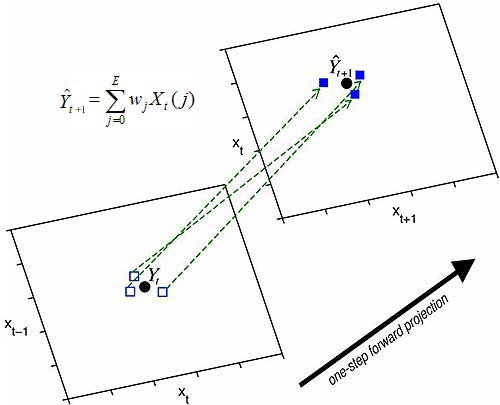
\includegraphics[width=\textwidth,height=0.95\textheight,keepaspectratio=true]{../images/simplex.jpg}
    \\
    {\scriptsize \texttt{http://simplex.ucsd.edu/} }
\end{center}
\end{frame}



\begin{frame}{S-mapping}
\begin{itemize}
    \item Sequentially locally weighted global linear maps (S-map)
    \item Designed to handle linear, locally nonlinear time series
    \item Similar to Simplex projection \\
        $\rightarrow$ But {\bf all} vectors are used for projection
    \item Weightings are again exponential
\end{itemize}
\vfill{\scriptsize Ref. \cite{Glaser2014}\cite{Sugihara1994} }
%NOTES
\note{
\vspace{-\baselineskip}
\begin{itemize}
    \item Sequentially locally weighted global linear maps (S-map)
    \item Similar to Simplex projection $\rightarrow$ But {\bf all} vectors are used for projection
    \item Weightings are again exponential
\end{itemize}
{\bf Procedure}
\begin{enumerate}
    \item Construct a ``library'' of time lag vectors $\{x_i\}$ of length $E$ and corresponding forward trajectories $\{y_i\}$
    \item Choose a state $x_t$ from which you wish to forecast the next system state $y_t$
    \item The estimation $\hat{y_t}$ is evaluated using
        \begin{equation*}
            \hat{y_t} = \sum_{j=0}^E c_t(j)x_t(j).
        \end{equation*}
        Here $c$ is obtained by solving the system $b=Ac$ where
        \begin{equation*}
            \begin{array}{rl}
                b(i)    & = w(||x_i-x_t||) y_i \\
                A(i,j)  & = w(||x_i-x_t||) x_i(j)
            \end{array}
        \end{equation*}
        where the weights are a function of Euclidean distance
        \begin{equation*}
            w(d) = e^{ \frac{-\theta d}{\bar{d}} }
        \end{equation*}
\end{enumerate}
}
\end{frame}



\begin{frame}
\begin{center}
    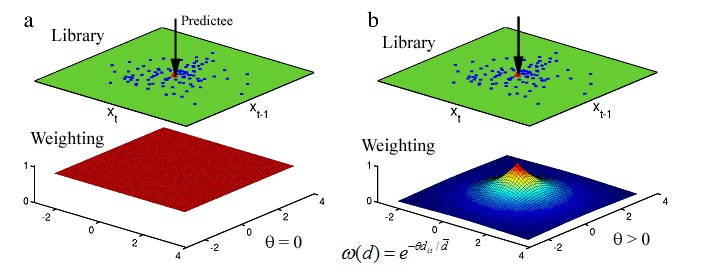
\includegraphics[width=\textwidth,height=0.95\textheight,keepaspectratio=true]{../images/smap.jpg}
    \\
    {\scriptsize \texttt{http://simplex.ucsd.edu/} }
\end{center}
\end{frame}



%--------------------------------------------------------------------------------------------------
\subsection{Mechanistic / semimechanistic}



\begin{frame}{Underlying dynamics - SIR}
\begin{itemize}
    \item Extensively used model in epidemiology
    \item Division into classes: {\bf S}usceptible-{\bf I}nfected-{\bf R}emoved
    \item Transition between states
        \begin{equation*}
            \begin{array}{rl}
                \frac{dS}{dt} & = - \frac{\beta I S}{N} \\
                \frac{dI}{dt} & = \frac{\beta I S}{N} - \gamma  \\
                \frac{dR}{dt} & = \gamma I
            \end{array}
        \end{equation*}
    \item Many extensions exist
    \begin{itemize}
        \item Additional classes
        \item Additional mechanistic terms
    \end{itemize}
\end{itemize}
%NOTES
\note{
\begin{itemize}
    \item Extensively used model in epidemiology
    \item Division into classes: {\bf S}usceptible-{\bf I}nfected-{\bf R}emoved
    \item Transition between states
        \begin{equation*}
            \begin{array}{rl}
                \frac{dS}{dt} & = - \frac{\beta I S}{N} \\
                \frac{dI}{dt} & = \frac{\beta I S}{N} - \gamma  \\
                \frac{dR}{dt} & = \gamma I
            \end{array}
        \end{equation*}
    \item Many extensions exist
    \begin{itemize}
        \item Additional classes
        \item Additional mechanistic terms
    \end{itemize}
    Can be used to test hypotheses
\end{itemize}
}
\end{frame}



\begin{frame}
\begin{center}
    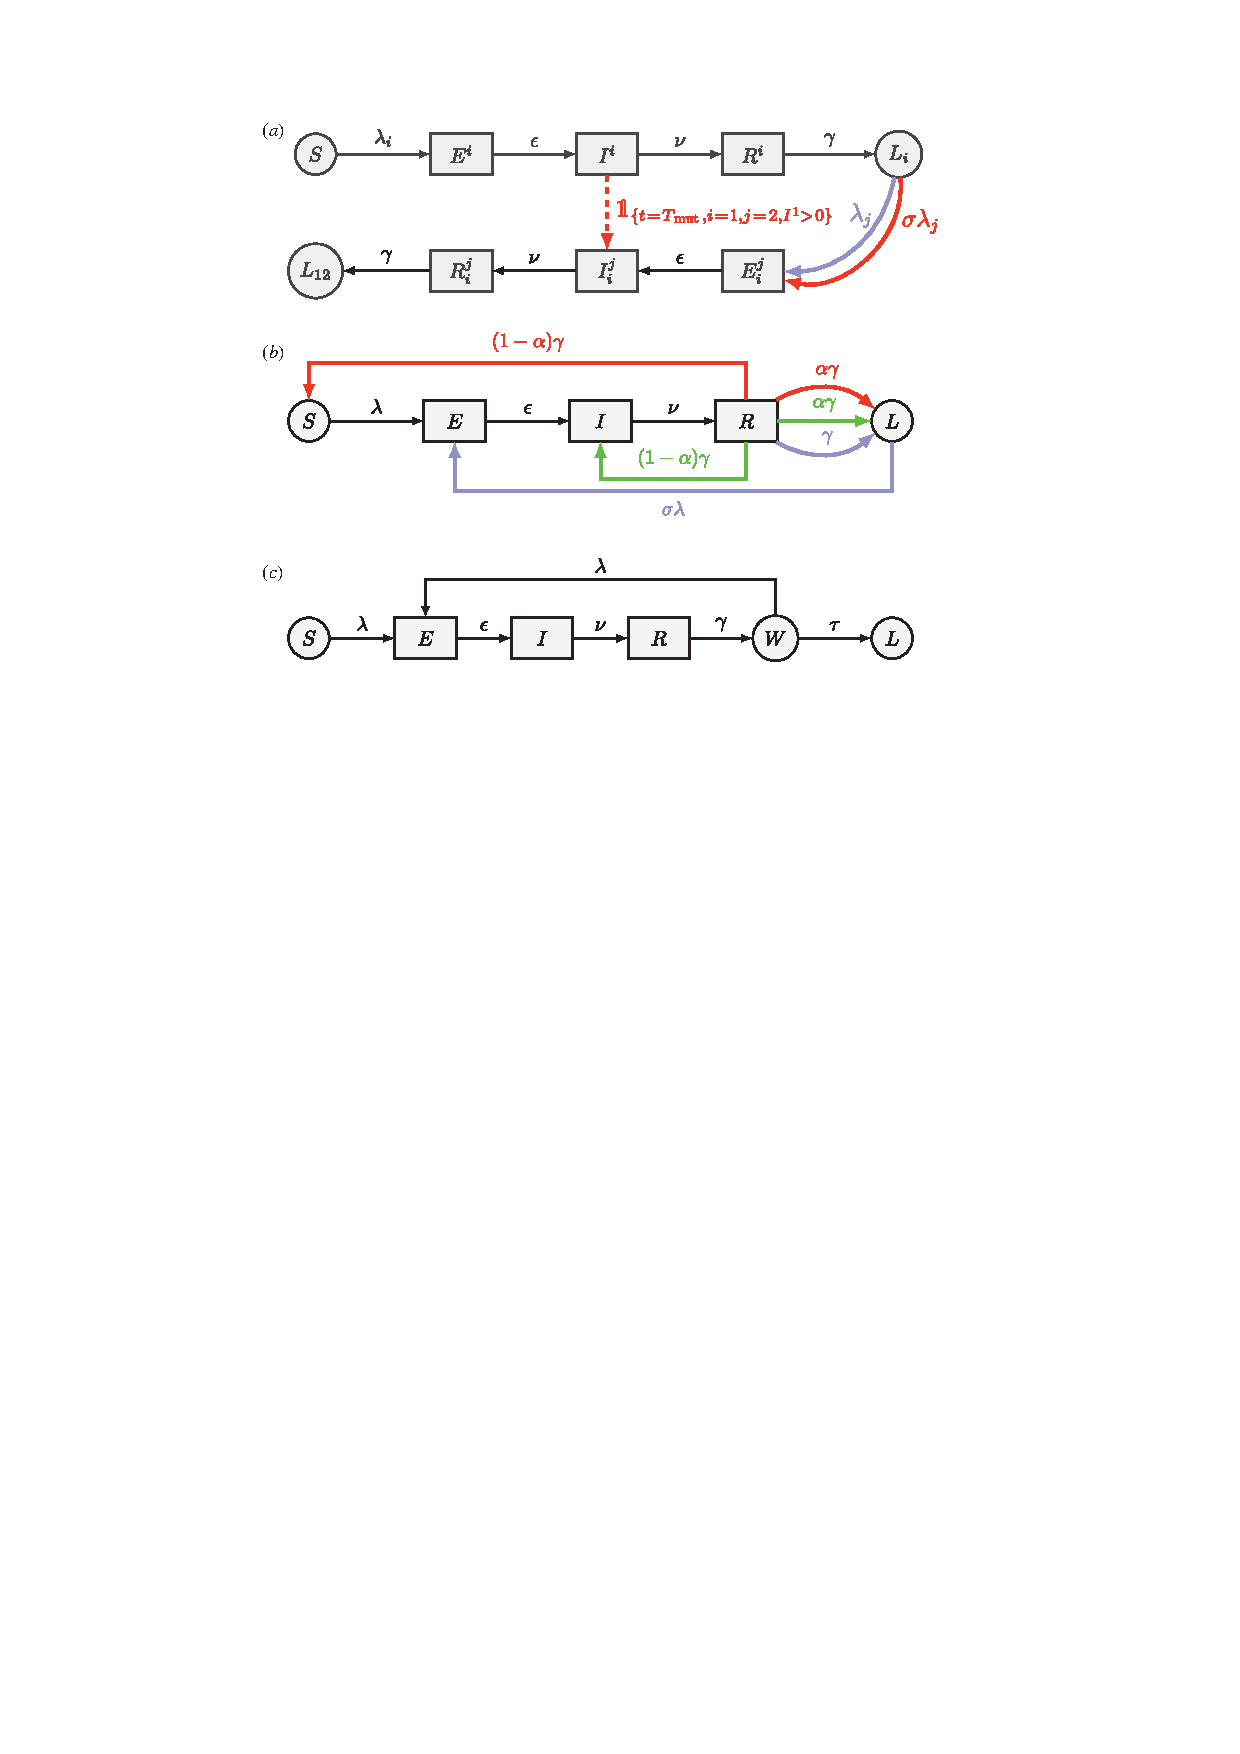
\includegraphics[width=\textwidth,height=0.9\textheight,keepaspectratio=true]{../images/seir_variations.pdf}
    \\
    {\scriptsize Camacho et al, 2011}\\
    \hfill{\scriptsize Ref. \cite{Graham2016} }
\end{center}
%NOTES
\note{
{\bf Example modification}
\begin{itemize}
    \item Part (c) hypothesis: window of reinfection
    \begin{itemize}
        \item long-term immunity takes time to develop
    \end{itemize}
    \item Three new classes added
    \begin{itemize}
        \item $E$ - exposed to virus, not yet infective
        \item $W$ - susceptible to reinfection, long-term immunity not developed
        \item $L$ - long term immunity developed
    \end{itemize}
\end{itemize}
}
\end{frame}



\begin{frame}{Parameter fitting}
\begin{itemize}
    \item SIR-based models {\it may} require many parameters to be estimated
    \begin{itemize}
    	\item Not a problem if statistical caution is exercised
    \end{itemize}
    \item Over-fitting a particular problem - can reduce forecasting ability
    \item More model complexity $=$ longer time series required
    \item Iterated filtering methods can estimate parameters in addition to producing forecasts
\end{itemize}
%NOTES
\note{
\begin{itemize}
    \item SIR-based models may require many parameters to be estimated
    \item Over-fitting a particular problem - can reduce forecasting ability
    \item More model complexity $=$ longer time series required
    \item Iterated filtering methods can estimate parameters in addition to producing forecasts
\end{itemize}
}
\end{frame}



\begin{frame}{Kalman filter}
\begin{itemize}
    \item Designed to operate on linear models, assumptions:
    \begin{itemize}
    	\item Underlying dynamics are linear
    	\item Error distributions are normal (or close to it)
    \end{itemize}
    \item Uses knowledge of underlying dynamics (ex. SIR model)
    \item Operation in cyclical phases
    \begin{itemize}
        \item Prediction $\rightarrow$ projection forward
        \item Update $\rightarrow$ observed data used to refine estimation mechanism
    \end{itemize}
\end{itemize}
%NOTES
\note{
\begin{itemize}
    \item Predictive method that operates on noisy data to produce optimal estimate of next system state
    \item Designed to operate on linear models
    \item Uses a model of expected system behaviour (for example a system of ODEs) to help with prediction
\end{itemize}
{\bf Prediction / update cycle}
\begin{itemize}
    \item Prediction
        \begin{align*}
            \hat{x}_{k|k-1} & = F_k \hat{x}_{k-1|k-1} + B_k u_k \\
            P_{k|k-1} & = F_k P_{k-1|k-1} F_k^T + Q_k
        \end{align*}
    \item Update
        \begin{align*}
            \tilde{y}_k & = z_k - H_k \hat{x}_{k|k-1}   \\
            S_k & = H_k P_{k|k-1} H_k^T + R_k \\
            K_k & = P_{k|k-1} H_k^T S_k^{-1} \\
            \hat{x}_{k|k} & = \hat{x}_{k|k-1} + K_k \tilde{y}_k \\
            P_{k|k} & = (I - K_k H_k) P_{k|k-1}
        \end{align*}
\end{itemize}
}
\end{frame}



\begin{frame}
\begin{center}
    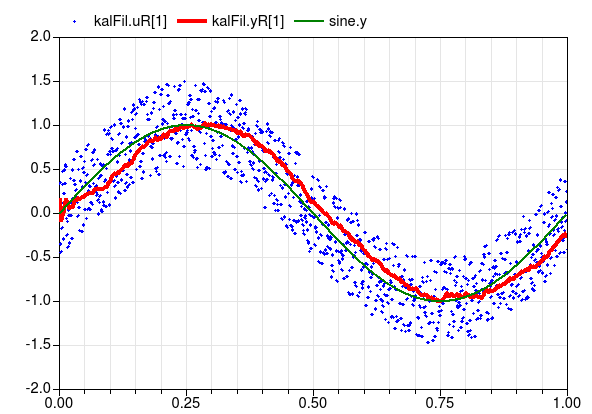
\includegraphics[width=\textwidth,height=0.95\textheight,keepaspectratio=true]{../images/KalmanFilter.png}
    \\
    {\scriptsize \texttt{http://simulationresearch.lbl.gov/modelica/releases/latest/help/
    Buildings\_Utilities\_IO\_Python27\_Examples.html} }
\end{center}
\end{frame}



\begin{frame}{Kalman filter extensions}
\begin{itemize}
    \item Extended Kalman filter ($EKF$)
        \begin{itemize}
            \item \alert{Linearises} about the estimate of current mean and covariance
        \end{itemize}
    \item Ensemble Kalman filter ($EnKF$) 
        \begin{itemize}
            \item Uses a \alert{cohort} of ensemble members, their sample mean and covariance
            \item Still assumes linear process / Gaussian distributions
            \item Useful for large number of parameters
        \end{itemize}
    \item Ensemble Adjustment Kalman filter ($EAKF$) 
	    \begin{itemize}
	        \item Combination of $EKF$ and $EnKF$ 
	        \begin{itemize}
	            \item \alert{Linearises} as in $EKF$
	            \item \alert{Ensemble members} as in $EnKF$
	        \end{itemize}
	    \end{itemize}
\end{itemize}
\vfill\hfill{\scriptsize Ref. \cite{Shaman2014} }
%NOTES
\note{
\begin{itemize}
    \item Extended Kalman filter ($EKF$)
        \begin{itemize}
            \item Linearises about the estimate of current mean and covariance
        \end{itemize}
    \item Ensemble Kalman filter ($EnKF$) 
        \begin{itemize}
            \item Uses a cohort of ensemble members, their sample mean and covariance
            \item Still assumes linear process / Gaussian distributions
            \item Useful for large number of parameters
        \end{itemize}
    \item Ensemble Adjustment Kalman filter ($EAKF$) 
        \begin{itemize}
            \item Combination of $EKF$ and $EnKF$ 
            \begin{itemize}
                \item Linearises as in $EKF$
                \item Ensemble members as in $EnKF$
            \end{itemize}
        \end{itemize}
\end{itemize}
}
\end{frame}



\begin{frame}{Particle filter}
\begin{itemize}
    \item Uses a set of particles, similar to $EnKF$ cohort
    \item Makes no assumption about the distributions involved in the system
    \item Particle importance using weights
    \item Problem: Particle degeneracy
    \begin{itemize}
        \item When one particle accumulates most of the weight
        \item Avoided via resampling at each iteration
    \end{itemize}
\end{itemize}
%NOTES
\note{
\begin{itemize}
    \item Uses a set of particles, similar to $EnKF$ cohort
    \item Makes no assumption about the distributions involved in the system
    \item Particle importance using weights
    \item Problem: Particle degeneracy
    \begin{itemize} \fontsize{7pt}{0em}\selectfont
        \item When one particle accumulates most of the weight
        \item Avoided via resampling at each iteration
    \end{itemize}
\end{itemize}
{\bf SIS} Sequential Importance sampling\\
\begin{itemize}
    \item Each of the $P$ particles at time $t$ consists of a weight-state pair $(w_t^{(i)},x_t^{(i)})$, such that $\sum\limits_{i=1}^{P} w_t^{(i)} = 1$
    \item Next system state (forecast) is given by the weighted average $\hat{x_t} = \sum\limits_{i=1}^{P} w_{t-1}^{(i)} f(x_{t-1}^{(i)})$
    \item After forecast, a new observation $x_t$ is assimilated and weights are recalculated based on how accurate the individual projections were
\end{itemize}
}
\end{frame}



\begin{frame}
\begin{center}
    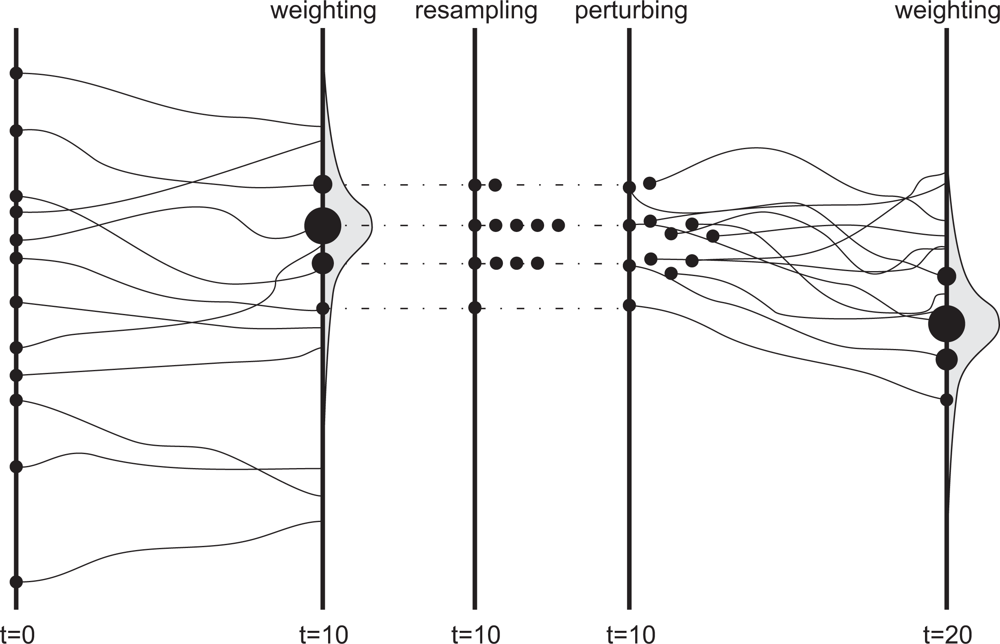
\includegraphics[width=\textwidth,height=0.9\textheight,keepaspectratio=true]{../images/particle.png}
    \\
    {\scriptsize \url{http://www.mdpi.com/sensors/sensors-12-16291/article_deploy/html/images/sensors-12-16291f2-1024.png} }
\end{center}
\end{frame}



\begin{frame}{Particle filter extensions}
\begin{itemize}
    \item Maximum likelihood via iterated filtering (MIF or IF1)
        \begin{itemize}
            \item Uses multiple rounds of particle filtering
            \item Stochastic perturbation of parameters
            \item Each round pushes the parameter estimates toward ML
        \end{itemize}
    \item Particle Markov chain Monte Carlo (pMCMC)
        \begin{itemize}
            \item Uses an MCMC method constrain model parameters
            \item Particle filter between each MCMC iteration
        \end{itemize}
    \item IF2 (MIF2)
    	\begin{itemize}
    		\item Evolution of MIF (IF1)
    		\item Uses stochastic perturbation as before, also data cloning
    		\item Looks to consistently outperform IF1 and pMCMC
    	\end{itemize}
\end{itemize}
\vfill{\scriptsize Ref. \cite{Ionides2015}\cite{Yang2014} }
%NOTES
\note{
\begin{itemize}
    \item Maximum likelihood via iterated filtering (MIF)
        \begin{itemize}
            \item Uses multiple rounds of particle filtering
            \item Each round pushes the parameter estimates toward ML
        \end{itemize}
    \item Particle Markov chain Monte Carlo (pMCMC)
        \begin{itemize}
            \item Uses an MCMC method constrain model parameters \\
            (typically the Metropolis-Hastings algorithm)
            \item Particle filter between each MCMC iteration
        \end{itemize}
\end{itemize}   
}
\end{frame}



%==================================================================================================
\section{Data assimilation}
%==================================================================================================




\begin{frame}{Incidence data}
\textbf{Primary Sources}
\begin{itemize}
    \item Google Flu Trends (GFT)
    \begin{itemize}
        \item Uses search trend data to infer incidence rates
        \item Almost instantaneous, but less accurate
        \item Currently up to 29 countries
    \end{itemize}
    \item Governments ex. Centres for Disease Control (CDC)
    \begin{itemize}
        \item Regional data (10 regions across the US)
        \item Broken down further by age
        \item More accurate than GFT, but lag of 1-2 weeks
    \end{itemize}
    \item WHO
\end{itemize}
\textbf{Social Media}
\begin{itemize}
	\item Twitter: Influenza, Korea, 2012 
	\item Social media and informal news: Haiti, Cholera, 2010
\end{itemize}
\vfill{\scriptsize Ref. \cite{Cook2011}\cite{Kim2013} }
%NOTES
\note{
\textbf{Primary Sources}
\begin{itemize}
    \item Google Flu Trends (GFT)
    \begin{itemize}
        \item Uses search trend data to infer incidence rates
        \item Almost instantaneous, but less accurate
        \item Currently up to 29 countries
    \end{itemize}
    \item Governments ex. Centres for Disease Control (CDC)
    \begin{itemize}
        \item Regional data (10 regions across the US)
        \item Broken down further by age
        \item More accurate than GFT, but lag of 1-2 weeks
    \end{itemize}
    \item WHO
\end{itemize}
\textbf{Social Media}
\begin{itemize}
	\item Twitter: Influenza, Korea, 2012 \\
			Very good estimates with ~40 keyword markers
	\item Social media and informal news: Haiti, Cholera, 2010 \\
			Not as good, ``Estimates of the reproductive number ranged from 1.54 to 6.89 (informal sources) and 1.27 to 3.72 (official sources) during the initial outbreak growth period, and 1.04 to 1.51 (informal) and 1.06 to 1.73''
\end{itemize}
}
\end{frame}



\begin{frame}{GFT vs CDC FluNet}
\begin{center}
	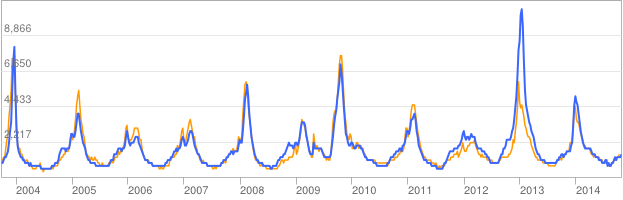
\includegraphics[width=0.9\textwidth,height=0.43\textheight,keepaspectratio=true]{../images/us_ili_gft_cdc.png}
    \\
    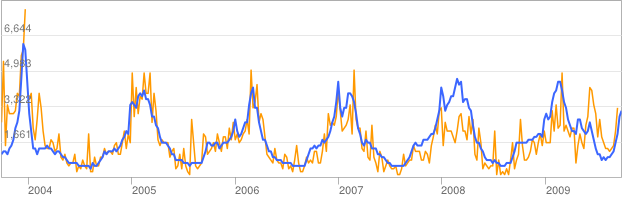
\includegraphics[width=0.9\textwidth,height=0.43\textheight,keepaspectratio=true]{../images/canada_ili_gft_phac.png}
    \\
    {\scriptsize \texttt{https://www.google.org/flutrends/about/how.html} }
\end{center}
%NOTES
\note{
\begin{itemize}
\item TOP
	\begin{itemize}
		\item US ILI
		\item Blue: GFT
		\item Green: Centres for Disease Control (CDC)
	\end{itemize}
\item BOTTOM
	\begin{itemize}
		\item Canada ILI
		\item Blue: GFT
		\item Green: Public Health Agency of Canada (PHAC)
	\end{itemize}
\end{itemize}
}
\end{frame}



\begin{frame}{Seasonality and Weather}
\begin{itemize}
    \item Nearly all infectious disease affected by seasonality
    \begin{itemize}
	    \item Contact
	    \item Susceptibility
	    \item Influx of susceptibles
	    \item Resevior dynamics / vector dynamics
    \end{itemize}
    \item Weather data sources
    \begin{itemize}
     	\item National Oceanic and Atmospheric Administration (NOAA)
     	\item NASA Jet Propulsion Laboratory (JPL)
     \end{itemize}
\end{itemize}
\vfill{\scriptsize Ref. \cite{Tamerius2013}\cite{Yang2014} }
%NOTES
\note{
\begin{itemize}
    \item Nearly all infectious disease affected by seasonality
    \begin{itemize}
	    \item Contact (people stay inside during cold weather)
	    \item Susceptibility (immunity already low in winter from colds, etc.)
	    \item Influx of susceptibles (schoolchildren)
	    \item Resevior dynamics / vector dynamics (mosquitoes more active in hotter weather)
    \end{itemize}
    \item Weather data sources
    \begin{itemize}
     	\item National Oceanic and Atmospheric Administration (NOAA)
     	\item NASA Jet Propulsion Laboratory (JPL)
     \end{itemize}
\end{itemize}
}
\end{frame}



\begin{frame}{ENSO}
\begin{itemize}
    \item {\bf E}l {\bf N}in\~{o} {\bf S}outhern {\bf O}cillation
    \item Sustained anomalous ocean surface temperature in the Pacific
    \item Unpredictable
    \item Many effects on local populations
    \item Relevant to epidemic outbreaks in Southeast Asian locales
    \begin{itemize}
        \item Cholera in Bangladesh
        \item Dengue fever in Singapore 
    \end{itemize}
\end{itemize}
\vfill{\scriptsize Ref. \cite{Hii2012}\cite{Reiner2012} }
%NOTES
\note{
    \begin{itemize}
        \item {\bf E}l {\bf N}in\~{o} {\bf S}outhern {\bf O}cillation
        \item Sustained anomalous ocean surface temperature in the Pacific
        \item Unpredictable
        \item Many effects on local populations
        \item Relevant to epidemic outbreaks in southern locales
        \begin{itemize}
            \item Cholera in Bangladesh (outbreaks in Dhaka highly correlated with ENSO)
            \item Malaria epidemics in South America (outbreaks in Colombia, Guyana, Peru, and Venezuela correlation with ENSO)
        \end{itemize}
    \end{itemize}
}
\end{frame}




%==================================================================================================
\section{Measuring prediction accuracy}
%==================================================================================================


\begin{frame}{Measuring Prediction Accuracy}
\begin{itemize}
	\item What to measure
	\begin{itemize}
		\item Peak timing / intensity
	    \item Magnitude
	    \item Duration
	\end{itemize}
    \item How to measure
    \begin{itemize}
    	\item Correlation coefficients
	    \item RMSE
	    \item Confidence intervals
	    \item Receiver operating characteristic (ROC) curves
	\end{itemize}
\end{itemize}
%NOTES
\note{
\begin{itemize}
	\item What to measure
	\begin{itemize}
		\item Peak timing / intensity
	    \item Magnitude
	    \item Duration
	\end{itemize}
    \item How to measure
    \begin{itemize}
    	\item Correlation coefficients (Pearson, etc.)
	    \item Root-Mean-Square Error (RMSE)
	    \item Confidence intervals
	    \item Receiver operating characteristic (ROC) curves
	    	\begin{itemize}
	    		\item Used to illustrate the performance of binary classifier system
	    		\item Obtained by plotting false positives against false negatives
	    	\end{itemize}
	\end{itemize}
\end{itemize}
}
\end{frame}


\begin{frame}{Model Criteria}
\begin{itemize}
	\item AIC - Akaike Information Criterion
	\begin{itemize}
		\item Measures relative model quality
		\item Rewards goodness-of-fit, penalizes for number of parameters
	\end{itemize}
	\item BIC - Bayesian Information Criterion
	\begin{itemize}
		\item Similar to AIC
		\item Tends to penalize many parameters more than AIC
	\end{itemize}
	\item DIC - Deviance Information Criterion
	\begin{itemize}
		\item Particularly useful when comparing MCMC-based models
	\end{itemize}
	\item WAIC - Watanabe-Akaike (widely applicable) Information Criterion
	\begin{itemize}
		\item More ``tuned'' to prediction
	\end{itemize}

\end{itemize}
%NOTES
\note{
	AIC and BIC require calculating the likelihood at its maximum over $\theta$

	WAIC uses the whole posterior density more effectively than DIC
}
\end{frame}


\begin{frame}[shrink=50]
\vspace{2\baselineskip}

\begin{multicols}{2}
\nocite{*}
\bibliographystyle{abbrv}
\bibliography{presentation}
\end{multicols}
\end{frame}

\plain{Thanks for coming!}{}

\plain{Questions?}{}




		
\end{document}